\subsection{Translation and ribosomal synthesis}

Lastly, we turn our attention to the process of translation. [expand on.]

\subsubsection{tRNA synthetases}

[expand on]

We begin by first estimating the number of tRNA synthetases.  \textit{E. coli} has roughly 3 x
10$^6$ proteins per cell, which for an average protein of 300 aa, amounts to the
formation of $\approx$ 10$^9$ peptide bonds. This value will also match the
number of amino-acyl tRNA that are required for protein synthesis, with the pool
of tRNA continuously recharging new amino acids by tRNA synthetases. At a rate
of charging of about 20 amino-acyl tRNA per second (BNID: 105279,
\cite{milo2010}), we find that cells have more than sufficient tRNA synthetases
to meet the ribosomal demand (\FIG{protein_synthesis}(A)).

\subsubsection{Protein synthesis}

[expand on]

If we consider an elongation rate of $\approx$ 15 peptide bonds per second
(BNID: 114271, \cite{milo2010, dai2016}), the formation of $\approx$ 10$^9$
peptide bonds would require about 1.5 x 10$^4$ ribosomes. This is indeed
consistent with the experimental data shown in \FIG{protein_synthesis}(B).

\begin{figure}
    \begin{fullwidth}
    \centering{
        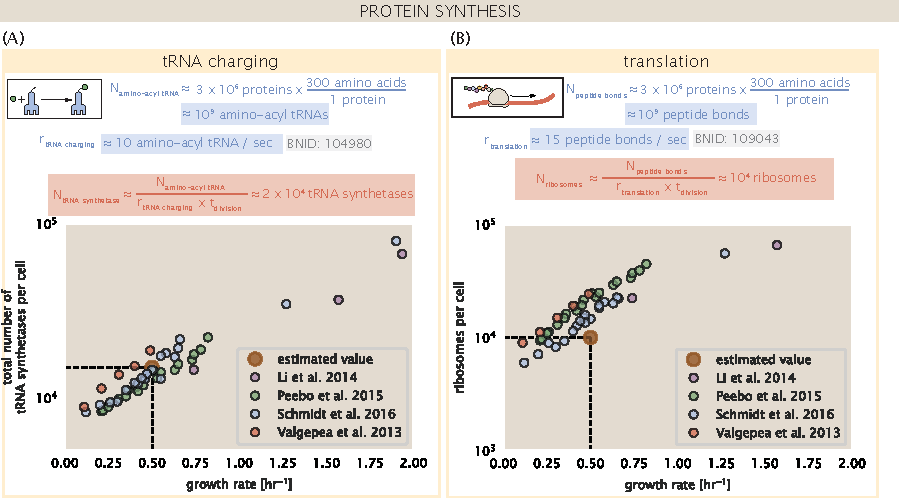
\includegraphics{main_figs/protein_synthesis.pdf}
        \caption{\textbf{Estimation of the required tRNA synthetases and
        ribosomes.} (A) Estimation for the
        number of tRNA synthetases that will supply the required amino acid
        demand. The sum of all tRNA synthetases copy numbers are plotted as a
        function of growth rate ([ArgS], [CysS], [GlnS], [GltX], [IleS], [LeuS],
        [ValS], [AlaS]$_2$, [AsnS]$_2$, [AspS]$_2$, [TyrS]$_2$, [TrpS]$_2$,
        [ThrS]$_2$, [SerS]$_2$, [ProS]$_2$, [PheS]$_2$[PheT]$_2$, [MetG]$_2$,
        [lysS]$_2$, [HisS]$_2$, [GlyS]$_2$[GlyQ]$_2$). (B) Estimation of the
        number of ribosomes required to synthesize 10$^9$ peptide bonds with an
        elongation rate of 15 peptide bonds per second. The
        average abundance of ribosomes is plotted as a function of growth rate.
        Our estimated values are shown for a growth rate of 0.5 hr$^{-1}$.}
    \label{fig:protein_synthesis}
    }
    \end{fullwidth}
\end{figure}


\subsubsection{Ribosomal synthesis}

So far our estimates have led to protein copy numbers that are consistent with
the proteomic data, or even in excess of what might be needed for each task
under limiting growth conditions. Even in our example of \textit{E. coli} grown
under different carbohydrate sources (\FIG{carbon_tport}(B)), it becomes clear
cells can utilize alternative carbon sources by inducing the expression of
additional membrane transporters and enzymes. Optimal resource allocation and
the role of ribosomal proteins have been an area of intense quantitative study
over the last decade by Hwa and others \citep{scott2010, hui2015}. From the
perspective of limiting growth, our earlier estimate of rRNA highlighted the
necessity for multiple copies of rRNA genes in order to make enough rRNA. For
\textit{E. coli}'s fastest growth rates at 2 hr$^{-1}$, the additional  demand
for rRNA is further supported by parallelized DNA replication and increased rRNA
gene dosage. This suggests the possibility that synthesis of ribosomes might
be rate limiting. While the transcriptional demand for the ribosomal proteins
is substantially lower than rRNA genes, since proteins can be translated from
relatively fewer mRNA, other ribosomal proteins like the translation elongation
factor EF-Tu also present a substantial burden. For EF-Tu  in particular, it is
the most highly expressed protein in \textit{E. coli} and is expressed from
multiple gene copies, tufA and tufB.

To gain some intuition into how translation may set the speed limit for bacterial
growth, we again consider the total number of peptide bonds that must be synthesized,
$N_\text{AA}$. Noting that cell mass grows exponentially \citep{godin2010}, we
can compute the number of amino acids to be polymerized as \begin{equation}
N_\text{AA} = \frac{r_t R}{\lambda}, \end{equation} where $\lambda$ is the cell
growth rate in s$^{-1}$, $r_t$ is the maximum translation rate in amino acids
per second, and $R$ is the average ribosome copy number per cell. Knowing the
number of peptide bods to be formed permits us to compute the
translation-limited growth rate as \begin{equation}
\lambda_\text{translation-limited} = \frac{r_t R}{N_\text{AA}}.
\end{equation}

Alternatively, since $N_{AA}$ is related to the total protein mass through the
molecular weight of each protein, we can also consider the growth rate in terms
of the fraction of the total proteome mass that is dedicated to ribosomal
protein mass. By making the approximation that an average amino acid has a
molecular weight of 110 Da (see \FIG{ribosome_limit}(A)), we can rewrite the
growth rate as,

\begin{equation}
\lambda_{\textrm{translation-limited}} \approx \frac{r_t}{L_R}  \Phi_R,
\label{eq:translation_limit_growth_rate}
\end{equation}
where $L_R$ is the total length in amino acids that make up a ribosome, and
$\Phi_R$ is the ribosomal mass fraction. This is plotted as a function of
ribosomal fraction $\Phi_R$ in \FIG{ribosome_limit}(A), where we take $L_R
\approx$ 7500 aa, corresponding to the length in amino acids for all ribosomal
subunits of the 50S and 30S complex (BNID: 101175, \citep{milo2010}). This
formulation assumes that the cell can transcribe the required amount of rRNA,
which appears reasonable for \textit{E. coli}, allowing us to
consider the inherent limit on growth set by the ribosome.

The growth rate defined by Equation \ref{eq:translation_limit_growth_rate}
reflects mass-balance under steady-state growth and has long provided a
rationalization to the apparent linear increase in \textit{E. coli}'s
ribosomal content as a function of growth rate \citep{Goldberger1979,
scott2010}. For our purposes, there are several important consequences of
this trend. Firstly, we note there is a maximum growth rate of $\lambda
\approx 6 \text{hr}^{-1}$, or doubling time of about 7 minutes (dashed line).
This growth rate can be viewed as an inherent maximum growth rate due to the
need for the cell to double the cell's entire ribosomal mass. Interestingly,
this limit is independent of the absolute number of ribosomes and is simply
given by time to translate an entire ribosome, $L_R/ r_t$. As shown in
\FIG{ribosome_limit}(B), we can reconcile this with the observation that in
order to double the average number of ribosomes, each ribosome must produce a
second ribosome. Unlike DNA replication or rRNA transcription, this is a
process that cannot be parallelized.

\begin{figure}
  \begin{fullwidth}
        \centering{
            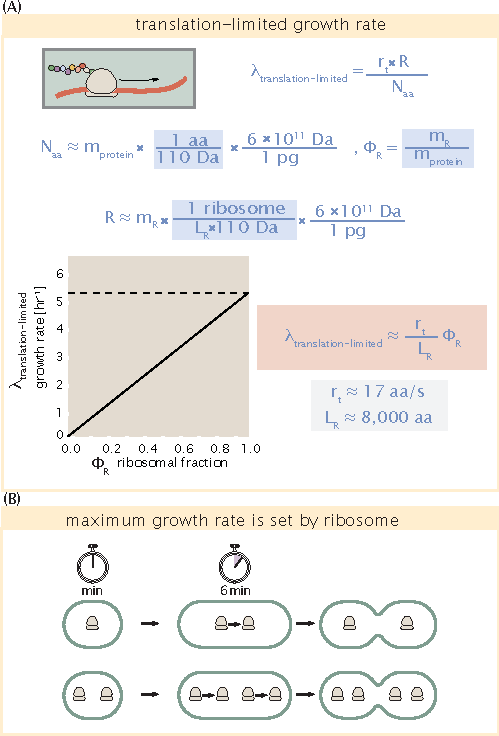
\includegraphics{main_figs/fig7_ribosome_growth_limit.pdf}
            \caption{\textbf{Translation-limited growth rate.} (A) Here we
            consider the translation-limited growth as a function of ribosomal
            fraction. By mass balance, the time required to double the entire
            proteome ($N_{AA}$ /$r_t$) sets the translation-limited
            growth rate, $\lambda_{\textrm{translation-limited}}$. Here $N_{aa}$
            is effectively the number of peptide bonds that must be translated,
            $r_t$ is the translation elongation rate, and $R$ is the number of
            ribosomes. This can also be re-written in terms of the ribosomal
            mass fraction $\Phi_R = m_R$ / $m_{\textrm{protein}}$, where $m_R$
            is the total ribosomal mass and $m_{\textrm{protein}}$ is the mass
            of all proteins in the cell. $L_R$ refers to the summed length of
            the ribosome in amino acids.
            $\lambda_{\textrm{translation-limited}}$ is plotted as a function of
            $\Phi_R$ (solid line). (B) The dashed line in part (A) identifies a
            maximum growth rate that is set by the ribosome. Specifically, this
            growth rate corresponds to the time required to  translation an
            entire ribosome, $L_R/ r_t$ . This is a result that is independent
            of the number of ribosomes in the cell as shown schematically here.
            (C)
            }
        \label{fig:ribosome_limit}
        }
  \end{fullwidth}
\end{figure}

For reasonable values of $\Phi_R$, between about 0.1 - 0.3 \citep{scott2010},
the maximum growth rate is in line with experimentally reported growth rates
around 0.5 - 2 hr$^{-1}$.
Importantly, in order for a cell to scale this growth
limit they \textit{must} increase their ribosomal abundance.
This can be achieved by either synthesizing more ribosomes or reducing the
fraction of non-ribosomal proteins. Reduction of non-ribosomal proteins is not
a straightforward task since (as we have found throughout our estimates) doubling a
cell requires many other enzymes and transporters. Increasing the absolute
ribosomal abundance in \textit{E. coli} will be limited by the number of
rRNA operons.

Here we again return to rRNA synthesis, but here consider the maximum rRNA that can
be produced at different growth rates.

[expand on.]
